% Chapter 2
\newpage
\part{Model} % Main chapter title

\label{chapter:model} % For referencing the chapter elsewhere, use \ref{Chapter1} 
$\frac{}{}$
%\lhead{Part  2. \emph{Model}} % This is for the header on each page - perhaps a shortened title
	
%----------------------------------------------------------------------------------------


As explained in the previous section, perhaps the most distinguishable aspect of high frequency trading is the speed with which agents can react to new market information. It is therefore essential that a model should capture this aspect, if it is to be used to draw generalized conclusions about the influence of high frequency trading in the markets.

The model consists of a market and agents. Agents and the market communicate by exchanging messages which all arrive one or several rounds after they are issued. A complete simulation consists of the several consecutive rounds. In each rounds, some agents submit orders, while others wait for new market information. Order messages arrive at the order books, and trades are executed when prices match.  The following sections will describe the model in detail.



\section{Model overview}

As has already been pointed out, the primary goal of the model is to simulate the presence of delays in communication between agents and then market. Furthermore, unlike previous models in which agents are divided into slow and fast traders, the model proposed in this work puts emphasis on modeling the real world scenario in which the latency with which the agents trade is an arbitrary period of time. As is discussed in section \ref{section:agents}, agents in this model are also divided into two groups of slow and fast traders, but since agents in either group have delays of an arbitrary number of simulation rounds, this division of the agents is much less strict than in previous models, such as \cite{keylist}, \cite{} and \cite{}.

Each round of the simulation corresponds to a period of real-time, but it is not particularly important to specify how long that period is. Instead, what matters is that there is a difference in speed between the agents. In other words, the important thing is that some agents are much faster than other agents. If one thinks of each round as a millisecond of real-time, one realizes that an agent simulating a human trader will require several thousands of simulation rounds to react to market news. On the other hand, fast algorithmic traders may only require a few rounds, making them several orders of magnitude faster than the slow traders. 

The model contains four main components and each of these will be described in the following subsections. 
\begin{itemize}
\item The stock which is traded by the agents
\item The market with a set of rules and an order book which handles transactions
\item The trading agents
\item The various messages that are passed between the agents and the market
\end{itemize}
Since there is relatively much to say on the agent strategies, section \ref{section:agents} has been devoted entirely to this subject.
Figure \ref{fig:agents_and_market} illustrates the relation between the agents and the market. 
\begin{figure}[htbp]
%issue 14
	\centering
		\includegraphics{Figures/manually_selected/model-graph.png}
		\rule{35em}{0.5pt}
	\caption{Diagram of the market model. Agents (blue and red nodes) have a various distances to the market (green node), as indicated by the different lengths of the edges.}
	\label{fig:agents_and_market}
\end{figure}

\subsection{Simulation rounds}
A complete simulation consists of executing $10^5$ consecutive rounds. Each round is composed by a number of steps, which can be divided into five parts as described below.
\begin{description}
\item[The round is initialized] Time is incremented and the fundamental price is updated. In this thesis, the only change to the fundamental price is at time $\round = \fundamentalshocktime$, where the fundamental price changes from $\fundamentalprice{0}$ to $\fundamentalaftershock = \fundamentalprice{0} - \fundamentalshocksize$.
\item[Arriving messages are dispatched to recipients] All messages with arrival time $\round{T}$ are delivered. Arriving transaction receipts delivered to the agents involved in the trades, and the portfolios of these agents are updated. Similarly, arriving orders and order cancellations are delivered to the market and placed in the order book message queue. Finally, all messages containing market information are received by the agents that requested the information. 
\item[Slow trader activity] The number of slow trader orders that arrive in this round is sampled from equation \ref{eq:poisson_distribution} and the orders are created using equation \ref{eq:slow_trader_price_determination}. The orders are instantly placed in the order book message queue.
\item[Fast trader activity] All HFT agents finishing evaluation of their strategies wake up and execute their decisions by sending out new orders containing orders and order cancellations. Each market maker \marketmaker{i} Each chartist \chartist{j} starts its hibernation period of \scwaitTimeBetweenTradingagent{j}.
\item[Order book is updated] All orders expiring this round are removed from the order book. Next, messages waiting in the message queue are processed in random order. Orders targeted by order cancellations are removed from the book, and transaction receipts are created for each pair of buy and sell orders with matching prices. After all messages have been processed, the best bid and ask prices, \bestbidprice{T} and \bestaskprice{T}, are set equal to the prices of the two most competitive remaining orders. In the case that no changed were made to the order book in round \round{T}, $\bestbidprice{T} = \bestbidprice{T-1}$ and $\bestaskprice{T} = \bestaskprice{T-1}$.
\end{description}


\subsection{The stock and its prices}
A single stock is traded in the market. The market uses a continuous double auction to match orders. As with anything that is traded in an auction, the traded asset cannot be said to have a single defining price. Instead, the value of the asset can be defined in (at least) three ways, as described below

\begin{description}
\item[Fundamental price] Often referred to as the ``true'' value of the stock. The fundamental price is establish by fundamental analysts, who try to estimate the stock price by analyzing the worth and wealth of the corporation that the stock represents. Hence, an accurate estimate of the fundamental price is arrived at only after careful (and time consuming) analysis. The fundamental price changes with the performance of the corporation, and is typically influenced by news. In this work, the fundamental price at round $\round{T}$is denoted $\fundamentalprice{T}$.
\item[Best offered prices] In the market, a stock is only worth as much as people are willing to pay for it. The value of the stock falls and rises according to what beliefs people hold about the worth of the stock. The best offered prices show what traders are currently willing to pay for the stock, and what price they are willing to sell for, and does not necessarily reflect the fundamental price. The best buy and sell price at round $\round{T}$ (e.g. the highest buy price and the lowest sell price) are denoted \bestbidprice{T} and \bestaskprice{T}.
\item[Traded price] Both of the two previous types of prices provide equally reasonable estimates of what the stock is actually worth. However, the willingness to trade does not always depend on the actual value of the stock. Sometimes traders need to sell their shares to acquire capital, and are therefore forced to lower the price at which they are willing to sell. Hence, a third way to estimate the value of a stock is to record the prices at which the stock was actually sold. The price of the $i$'th transaction in round $\round{T}$ is denoted $\tradeprice{T}{i}$. The double auction works in such a way that trades are always executed at the best prices currently existing in the order book at the time of the trade. However, since the market depth is finite, a large quantity of orders will move \bestaskprice{T} and \bestbidprice{T}, and consequently it frequently happens that $\tradeprice{N}{i} \neq \tradeprice{N}{i+1}$.
\end{description}

The fundamental price is used as the benchmark price for the slow traders (also called the fundamentalists), the best buy/sell prices are used by the fast market makers, and the traded price is used by the fast chartists. See section \ref{section:agents} for more details. Whether or not one type of strategy is more accurate than the other, it is a fact that both types are employed by traders. Hence, a model of such an environment needs to include all three types of prices.



\subsection{Order book}
The order book is a record of all unmatched orders for a single stock. Since any buy-and sell orders submitted at the same price will cause a trade to be executed, and the matched orders to subsequently be removed, there must at any point of time during the simulation be a non-negative price difference between the sell order with he lowest price and the buy order with the highest price. This difference is called the \textit{spread}, and is denoted as follows
\begin{equation}\label{equation:spread_definition}
\spread{\round{T}} = \bestaskprice{\round{T}} - \bestbidprice{\round{T}}
\end{equation}
where \bestaskprice{\round{T}}{} and \bestbidprice{\round{T}}{} are the best ask and bid prices in round \round{T}.

\begin{table}
\centering
\begin{tabular}{l|c|r}
Sell orders & Price & Buy orders\\
\midrule
& \vdots & \\
22 & 9994 &\\
26 & 9993 &\\
13 & 9992 &\\
10 & 9991 &\\ 
{}&{}&{}\\
& 9988& 12\\
& 9987& 10\\
& 9986& 16\\
& 9985& 25\\
& \vdots &\\
\end{tabular}
\caption{Example of an order book in the price range near the best buy/sell prices}
\label{table:orderbook_example}
\end{table}



\subsubsection{Price updating}
Each time an order is added or removed, the order book has to update the best \bid{} and \ask{} prices. Since it often happens that several orders arrive in the same round, the order book spread can fluctuate within a single round. However, since one round is considered the minimum quantum of time,  these within-round fluctuations are not recorded in the order book history. Instead, after all orders have been processed, the resulting best \bid{} and \ask{} prices are registered as the best prices for that round. Agents that look at the market will therefore only be able to see the state of the order book after the book has finished processing all price changes due to the arrival or removal of orders. The subscript denoting time in equation \ref{equation:spread_definition} therefore refers to the prices at the end of that round. 

When no orders arrive or are removed from the order book, the prices are updated as 
$\bestaskprice{{\round{T} + 1}} = \bestaskprice{\round{T}}$ and $\bestbidprice{{\round{T} + 1}} = \bestbidprice{\round{T}}$. Since orders can be removed due to cancellations or because they expire, the order in which incoming messages is processed matters to the outcome of \bestaskprice{\round{T}} and \bestbidprice{\round{T}}. Messages are therefore processed in random orders, so that no agent is favored.



\subsubsection{Order matching}\label{section:order_matching}
When a trade is executed between orders $o_1$ and $o_2$, the traded volume is 
\begin{equation}
\Delta v = \min (v_{o_1}, v_{o_1}) \nonumber
\end{equation}
If $v_{o_1} = v_{o_2}$ the orders are \textit{fully matched}, and both are removed from the order book. In the case of a \textit{partial match}, that is, if the volume of one order is larger than the volume of the other, then the order with the smaller volume is removed, and the volume of the other order is subtracted by $\Delta v$. The price of the transaction is the price of the market order which was already in the book. 

Each agent knows the volume of every order that it submitted, when the order was dispatched. However, when an order is partially filled by a matching but smaller order, the volume of the order at the market changes. Since it takes time for the order to be transmitted for the agent to the market, the agent cannot immediately update its knowledge of the order volume. In this case the order has one volume at the agent side and another in the market side. The momentary disparity of agent market side and agent side volumes can have several consequences, such as agents short-selling without, agents submitting cancellations for orders which have already been filled. Rules that handle these situations are described in section \ref{section_marketRules}. Unlike volumes, the price of a standing market order does not change, and hence the situation of a disparity between market- and agent-side price knowledge does not occur.





\subsection{Messages}
All communication between the market and agents is transmitted in messages and all messages take a non-zero number of rounds to arrive. This means that no information is transmitted instantly between agent and market. The latency between any agent and the market is constant throughout the simulation, but different for each agent. The delay between market maker \marketmaker{i} and the market is \ssmmlatencyagent{i}, and the distance between chartist \chartist{j} and the market is \sclatencyagent{j}. All latencies between agents and markets are non-negative integers. A message created in round $\round{T}$ by an agent with a latency of $\lambda$ rounds to the market with arrive at the market in round $\round = \round{T} + \lambda$. Several message types were implemented in order to accommodate the various types of communication.

\begin{figure}[htbp]
%issue 14
	\centering
		
\includegraphics{Figures/Electron.pdf}
		\rule{35em}{0.5pt}
	\caption{}
	\label{fig:information_exchange}
\end{figure}


\subsubsection{Market information}
One of the key points of simulating delays is that agents always trade on old information. Before an agent can evaluate its strategy, it has to request the most recent market information. In a model without delays, an agent would simply receive the state of the market in the current round, but when information is delayed the process is somewhat more cumbersome. First the agent sends off a request to obtain the information about the market state. When the request arrives at the market some rounds later, the market serves the request and by sending back another message containing the information. The contents of this message depends on the agent strategy, as the various agent strategies require different information. 
In the case of a single market, it is reasonable to simplify the model such that the market serves the request instantaneously, since any delay inherent in the market is common for all agents. 
After a further delay, the message containing the market state finally arrives at the agent, and the agent can then start evaluating its strategy. Figure \ref{fig:information_exchange} summarizes the procedure.

This is analogous to how 
\begin{figure}[htbp]
	\centering
		
\includegraphics{Figures/Electron.pdf}
		\rule{35em}{0.5pt}
	\caption{When an agent wants to submit an order it has to go through several steps of interaction with the market. The process is comparable to how real traders communicate with markets via a network, such as the Internet.}
	\label{fig:information_exchange}
\end{figure}


\subsubsection{Orders}
An order is a message which is sent from an agent to a market when the agent has decided to trade. An order is an offer to buy or sell a specified number of shares at a certain price at a certain market. Orders can either be limit orders or market orders. A limit order will only result in a trade to be executed if there is a matching order when it arrives to the market. A market order will stay in the order book until a matching order arrives, or until it expires after a number of rounds set by the submitting agent. 

When an agent creates an order, the agent first of all decides on whether the order is a sell order or a buy order, a limit order or a market order. The agent also specifies the price and the volume of the order. Details on how each type of agent does this can be found in section \ref{section:agents}. Once the price has been decided upon, it stays fixed for the duration of the order lifetime. On the other hand, the volume does not remain constant. If the agent submits a market order, the order sits in the order book for a number of rounds before it expires. If during that time there is an order on the other side of the book with the same price, a trade is executed. If the two orders involved in the trade do not have identical orders, a partial match occurs (see section \ref{section:order_matching}), and the volume of the largest order is updated. When this happens, the market instantly sends out a transaction receipt to the agent. However, since it takes time for the receipt to reach the agent, there is a period of time during which the agent is unaware that the order that it places has been involved in a trade. Hence, every order has two simultaneous volumes. The market-side volume specifies the actual remaining volume of the order as it is in the order book, while the agent-side volume reflect what the agent knows about the order. Whenever an order is involved in a trade, a discrepancy between the market-side volume and the agent-side volume occurs, and is resolved as the transaction receipt reaches the agent. 
%This discrepancy between the market-side and the agent-side volumes can cause agents conflicts. For instance, an agent holding order $O_1$ at the market might observe a change in the best price due to a trade not involving $O_1$. The agent might decide to cancel $O_1$, and submit another order $O_2$ at the new best price. However,iIf the agent decides to do so at any point of time during which a transaction receipt is traveling towards the agent, the new order submitted by the  
%While the market-side order can be thought of as the ``true'' volume, the agent does not know this, and therefore bases its trade decision on the agent-side volume.


\subsubsection{Transaction receipts}
When two orders match, a receipt is sent to each of the two agents involved in the trade. The seller receives a receipt specifying the number of shares that it has to deliver, and the buyer gets a receipt for the amount of cash to be paid. Because of the transmission delay, the agents to not update their portfolios when the trade actually happens, but when they receive the receipt. In the case that an agent does not have enough shares or cash in its portfolio, the agent is allowed to borrow the necessary assets, thus bringing its portfolio into negative. An agent cannot submit new sell orders while holding a negative number of shares. Similarly, an agent cannot submit any new buy orders while having a negative amount of cash. In the case that the agent has neither cash nor shares, it simply becomes inactive.

\subsubsection{Order cancellations}
It can happen that an agent wants to change a previously submitted order, or cancel it entirely. In fact, this is what the market maker agent does frequently, as described in section \ref{section:market_maker}. In this case, the agent issues a message to the market requesting that the order should be removed. Due to the presence of delays, the agent's order might be filled before the cancellation reaches the market, in which case the market will ignore the request to cancel.

\subsection{Market rules for short selling}
Although some market do allow deliberate short selling, this practice is not allowed in the simulation. That is, an agent is not allowed to place a sell order for more stock than it has in its portfolio at the time it places the order. However, due to the presence of delays, it can happen that an agent is required to deliver on a sell order for more stocks than it holds when notified of the order. A sequence of events which causes this to happen is  illustrated on figure \ref{fig:short_selling}. The agent who is short is required to deliver the stocks, and thus goes into negative on its portfolio, and has to buy back the stocks before it can place further sell orders. Although the sequence of events shown in figure \ref{fig:short_selling} may seem unlikely, it did in fact occur frequently, making it necessary to implement handling of this special case. 
\begin{figure}[htbp]
	\centering
		
\includegraphics{Figures/Electron.pdf}
		\rule{35em}{0.5pt}
	\caption{The HFT agent submits a sell order for 100 stocks, and another agent submits a price-matching buy order which fills the sell order. Before the transaction receipt reaches the seller, the seller decides to cancel the order, and submit another order at a different price. When the transaction receipt reaches the seller, the agent promptly sends out a cancellation of its second sell order, as it knows it cannot fulfill the order. However, before the cancellation reaches the market, a third agent fills the sell order, and a receipt is send to the seller who ends up being short.}
	\label{fig:short_selling}
\end{figure}



\section{Agents}\label{section:agents}

A taxonomy of agents which is frequently found in the literature dealing with the speed of traders, is a division of traders into a group of fast agents and a group of slow agents (\cite{foucault2012news, hoffmann2012dynamic, mcinish2012strategic}). While the model proposed in this work uses a similar division, it is less rigid as agents in each group can have arbitrarily large (or small) latencies. Rather, the division of agents into slow and fast traders is intended to capture traits of traders in the real world. Hence, the slow traders are meant to model human traders, which tend to react slowly to market information but are capable of interpreting world events that influence the stock price. The slow traders are also intended to model algorithmic traders which use human-like strategies, but do not benefit from co-location. On the other hand, the fast traders, also referred to as HFTs, are intended to model algorithmic traders which do make use of co-location \cite{brogaard2013trading} and use strategies of a lower complexity and variety compared to human traders \cite{chaboud2009rise}.  In this report, HFT agents will often be referred to as being ``fast'' or ``slow'' when talking about agents with small or large latencies to the market. While an agent's latency to the market is unrelated to how fast or slow an agent is (other parameters, such as \ssmmthinkagent{i}, \scthinkagent{i} is more related to an agent's speed), the agent's latency does determine the delay with which the agent received market information. By fast and slow agents is therefore meant agents that can or cannot respond quickly to new market events.

Another way to group agents is by the nature of their strategy. In financial markets, every trader is supposed to have access to the same information. However, two traders might disagree on the meaning of some piece of information. The way in which a trader evaluates market information and reaches a conclusion on how to trade is called a strategy. While any function which takes some information relevant to the market as input and gives a decision of how to trade (or not trade) can be termed a strategy, it is useful to divide strategies into two broad categories. In the first category are strategies which are dubbed chartist strategies, which basically tries to extrapolate on the past price movements. An agent modeling this behavior is described in section \ref{section:hft_chartist}. In the other category are strategies which are based on some analysis of the true value of the stock, called the fundamental value. This behavior is replicated as described in section \ref{section:slow_traders}. The market maker strategy explained in section \ref{section:market_maker} does not really belong to neither of these two groups, as the agent neither tries to extrapolate on past data, not use fundamental analysis for price determination. The above classification of agents is by far meant to be definitive. 





\subsection{Slow traders}\label{section:slow_traders}
The slow trader model used in this work is inspired by the stylized trader model used in \cite{chiwang2013investigating, chiarella2009impact, gsell2008assessing}. However, due to the fundamental differences in the way that the simulation works, the model has been modified significantly. 
%Since the stylized trader model is so predominant in the market simulation literature (see \cite{asd}, \cite{asd} etc.), we feel that we need to justify our choice of not using it. 
The idea of the model is that there are three basic trading strategies techniques that any human trader trader mixes to form his own personal strategy. 
\begin{description}
\item[Fundamental analysis] Traders subscribing to this way of thinking believe that they can know the true value of a stock by estimating the fundamental price (see section \ref{section:fundamental_price}). Furthermore, such traders believe that any deviation from the fundamental price is due to other traders misinterpreting the market, and that such deviations will eventually disappear. In other words, given enough time, the traded price will converge towards the fundamental price. 
\item[Technical analysis] Traders using technical analysis do not care whether or not the stock is over valued. Instead, they believe that they can predict future price movements from past data. Traditional technical analyst approaches extrapolates on price movements by using simple mathematical models and a good deal of heuristics.
\item[Noise trading] Some traders are in possession of insider knowledge, which means that they think that they know something about the stock that others do not. They use this information to trade the stock, for better or for worse. Such traders were dubbed noise traders, since it is highly unlikely that any one individual would come in possession of information which actually gives that person an advantage in the market. Any such belief is therefore naive, and might as well inflict a loss on the agent than generate a profit.
\end{description}

 The orders submitted the stylized traders throughout the run of the simulation should be thought of as being submitted by a variety of different agents, all observing the same historical data, but interpreting it differently using different strategies. In other words, the model for the slow traders proposed in this work should thought of as representing a group of traders \cite{drogoul2003multi}. Hence, even though all the slow traders are fundamentalists, they all have slightly differing opinions on what the fundamental price actually is at any given moment. This difference in opinion is modeled by adding normally distributed noise to the price estimate, as described below. In this model the fundamental and noise trader parts of the stylized trader strategy are preserved, but the chartist behavior is removes. Most chartist strategies operate on a timescale of days to weeks to months. However, the simulation proposed in this work merely simulates a few minutes of real-time\footnote{This is not entirely accurate as each round can be interpreted as an arbitrary length of real-time. However, since we are interested in what phenomena occur when we have some agents which are several orders of magnitude faster than other agents, we need a high time resolution, effectively capping the length of real-time which can be simulated}. Any chartist strategy based on the entire history of price movement over a long period of time will simply be too sluggish to follow with the high frequency price fluctuations occurring within the simulation. In other words, to a slow trader that relies heavily on the chartists part of the stylized trader strategy and calculates the moving average of the traded price over a period of days or months, any price changes that take place during a few seconds will hardly register at all. Even to relatively fast stylized traders that rely of minute-by-minute price changes, the time span simulation by the model is so short that the price changes that take place during the simulation will be smoothed out by trader's moving average calculation. This does not mean that the model neglects to recognize the fact that slow trader chartists do exist, but since these traders base their price estimates on price data from the past days, weeks or even months, it is not possible to simulate these strategies directly as it would require an exorbitant number of simulation rounds. Instead, the presence of chartists are modeled by adding fast agents using a short-term chartist strategy, which is described in section \ref{section:hft_chartist}. 
 

%Instead, the contributions of long term chartists is modeled as simply additive gaussian noise. While this may indeed be an over-simplification, this approach is justified if assuming that the slow trader chartists 


 \subsubsection{Strategy} 
The slow trader observed the market with a delay of \stlatency. Hence, in round $\round{T}$, the slow trader knows the price of the true fundamental in round $\round{T} - \stlatency$, which will be dubbed $\fundamentalprice{T-\stlatency}$. The noisy part of the agent strategy \cite{hommes2006heterogeneous} adds a normally distributed number to $\fundamentalprice{T-\stlatency}$, such that the fundamental price estimated by the slow trader is 
\begin{equation}
\fundamentalprice{\text{est}} = \fundamentalprice{T-\stlatency} + \stnoise
\end{equation}
where $\stnoise \sim \mathcal{N}(\stnoisemu, \stnoises)$. The trader also observed the the best prices in the order book $\bestaskprice{\round{T} - \stlatency}$ and $\bestbidprice{\round{T} - \stlatency}$. The slow trader uses his estimate of the fundamental price to determine whether to buy or sell, and at which price. 
\begin{flalign*}
&\text{Place a buy order if} & & \fundamentalprice{\text{est}} > \bestbidprice{\round{T} - \stlatency}  && \text{at buy price} & & p_\text{b} = \bestbidprice{\round{T} - \stlatency} + C\\
&\text{Place a sell order if}  & & \fundamentalprice{\text{est}} < \bestaskprice{\round{T} - \stlatency}  && \text{at sell price} & & p_\text{s} = \bestaskprice{\round{T} - \stlatency} + C
\end{flalign*}
Hence, the slow trader will try to acquire shares when he believes that the fundamental price is higher than the current best bid, and sell shares if the fundamental price is lower than the current best ask price. If the estimated fundamental price is between the delayed bid/ask prices, that is if $\bestbidprice{\round{T} - \stlatency} < \fundamentalprice{\text{est}} < \bestaskprice{\round{T} - \stlatency}$, the agent chooses to place a sell or buy order with equal probability with the same prices as in the above equations.


\subsubsection{Order arrival}
The arrival of orders from slow traders is modeled as a Poisson process, as this is a model which has been used in other works as well ( see \cite{cincotti2006waiting} and \cite{amihud1980dealership}). Hence, such that the number of new orders any round \round{T} is a random variable, $\kappa_T$ sampled from a Poisson distribution:
\begin{equation}\label{eq:poisson_distribution}
\kappa_T \sim Pois(\storderarrivalrate)
\end{equation}
In \cite{amihud1980dealership} the number of buy order and the number of sell orders are distributed according to two separate Poisson processes. In this work the market is assumed to be in a stable state prior to the shock to the fundamental price, and hence the average number of arriving buy orders is assumed to be the same as the average number of sell orders. Therefore a single Poisson process is used to obtain the number of newly arriving orders, and these orders are then divided into sell and buy orders with equal probability. Furthermore, since the model only simulated a short span of time after the shock, it is reasonable to assume that \avrstorders{} is constant as the population of slow traders can be assumed not to be exhibit any herding behavior which might occur over longer periods of time \cite{herding}.


\subsection{HFT Market makers}\label{section:market_maker}
Market making is the term used for strategies in which the trader is simultaneously active on both sides of the order book. The trader attempts to make a profit by submitting sell orders at price $\bestaskprice{\delta}$ and buy order at price $\bestbidprice{\delta}$, making sure that $\bestaskprice{\delta} > \bestbidprice{\delta}$. Here, $\delta$ is used to indicate the the best bid and ask prices that the market maker is trying to match are delayed according to the total latency of the agent. The difference between the bid price and the ask price is the market maker's spread. Trading with a small spread makes the market maker competitive by attracting orders from other traders, but also makes the market maker incur risk by increasing the risk of trading at sub-optimal prices in the case of sudden price fluctuations. 

\subsubsection{Strategy outline}
The market maker aggressively tries to maintain orders at the best buy and sell prices. As other agents submit orders, the buy and sell prices move up and down, and the difference between the best buy price and the best sell price, also known as the spread, increases and decreases accordingly. Since the agent tries to maximize its own profit, it chooses prices which maximizes the spread. Hence, when the spread increases, the agent is happy to let it do so, as it can then buy and sell with a larger profit on each unit of the traded asset. On the other hand, when the spread decreases, the agent also changes its prices in order to attract trades which would otherwise go to other agents. However, if the spread becomes too small, the profit on each unit of the traded asset becomes too small to justify the risk of holding stock which might suddenly drop in value. Therefore the strategy employed by the agent specifies a minimum accepted spread at which the agent is willing to trade. When the market maker receives a notification that one of its orders has been filled, it immediately uses the most recent locally known market information to submit a new order. For the sake of simplicity, each market maker agent is allowed to have a single market order at each side of the order book. The agent can therefore not stack orders on either side of the order book. 

\subsubsection{Parameterization}
The market maker behavior is controlled by the following parameters
\begin{description}
\item[Minimum spread] The parameter \ssmmminspreadagent{i} controls the smallest spread at which the agent will trade. The agent will never submit orders such that the price difference between his standing buy and sell orders is smaller than \ssmmlatencyagent{}.
\item[Order volume] Market maker \marketmaker{i} submits orders with volume \ssmmordervolumeagent{j}. Since the market maker tries to maintain standing orders at the orderbook for as much of the time as possible, \ssmmordervolumeagent{i} is usually chosen to be fairly large. \ssmmlatencyagent{i} is selected when the agent is created, and is constant throughout the simulation.
\end{description}


\subsubsection{Price determination}
When the agent receives the delayed trade prices from the market, the spread can either increase or decrease relative to the agent's previously known prices. In the former case, the agent always updates its prices to follow the widening gap between the buy side and the sell side. When the spread decreases, the strategy requires the agent to check that the minimum spread condition, that is whether or not $s_{r} < \ssmmminspreadagent{i}$, where $s_{r}$ is spread the calculated from the trade prices that the agent has just \textit{received}. If the condition is not violated, then the agent can freely update prices to follow the current trade prices. If the condition is violated, then the agent determines the trade price by the following equations. $p^b_n$ and $p^s_n$ are the \textit{new} buy and sell prices, $p^b_r$ and $p^s_r$ are the best buy and sell prices that the agent currently knows of, and $\Delta p^b$ and $\Delta p^s$ are the absolute differences of the prices:
 that is $\Delta p^b = \lvert p^b_n - p^b_r \rvert$ and $\Delta p^s = \lvert p^s_n - p^s_r \rvert$.
\begin{align}
& \begin{array}{l}
p^b_n = p^b_r\\
p^s_n = p^b_r + \ssmmminspreadagent{i}
\end{array}
\bigg\}
&\text{ when }& &
& p^b_n = p^b_r, p^s_r < p^s_r
\\
& \begin{array}{l}
p^b_n = p^s_r - s_m\\
p^s_n = p^s_r
\end{array}
\bigg\}
&\text{ when }& &
&\begin{array}{l}
p^b_n > p^b_r\\
p^s_n = p^s_r
\end{array}
p^b_n > p^b_r,  p^s_n = p^s_r
\\
& \begin{array}{l}
p^b_n=p^s_r-(s_m-s_r)\frac{\Delta p^b}{\Delta p^b+\Delta p^s}\\
p^s_n=p^b_r+(s_m-s_r)\frac{\Delta p^s}{\Delta p^b+\Delta p^s}
\end{array}
\bigg\}\label{eq_bothSidePriceUpdate}
&\text{ when }& &
&\begin{array}{l}
p^b_n > p^b_r\\
p^s_n < p^s_r
\end{array}
\end{align}
The equations in \ref{eq_bothSidePriceUpdate} are used in the case where the both the buy and sell prices moves so that the spread becomes smaller than $s_m$. The equations are designed so that the agent will change its trade price in proportion to the change on either side of the book. For instance, if the buy price suddenly increases a lot while the sell side only decreases a bit, such that $s_t < s<m$, the agent will increase his own buy side price by a lot and decrease his sell price side by a little, so that the spread of between the new orders are $s_n = p^s_n - p^b_n = s_m$.

Figure \ref{figure:marketmaker_strategy} shows three simple examples of how the market maker attempts to follow the best market prices. $\delta$ is used to designate the total amount of time that elapses between the prices at the market change and until the market maker can have a new order at the market, and thus includes both the delay from $\ssmmlatencyagent{}$ and $\ssmmthinkagent{}$. 

In the first case, the spread increases, and the market updates its own prices to follow the increasing spread. In round two to eight, the market maker is selling at a price of 13 ticks, while the best market sell price is two ticks higher at 15 ticks. This means that the delay causes the market maker to momentarily sell at sub-optimal prices, and hence would makes 2 ticks less of profit per share if its order is filled before the market makers new order reaches the market. 

In the second example, the spread decreases, and the market maker again its prices to a lower spread in order to stay competitive. In this case, the delay in the market maker's ability to react to the market events causes the market maker to momentarily be less competitive than possible, causing a risk of losing trades. 

In the third and fourth examples, the minimum spread parameter \ssmmminspreadagent{} is seen to force the market maker to trade at sub-optimal prices, as the spread narrows below four ticks.

\begin{figure}
\centering
%issue 11
\subcaptionbox{}
[0.49\linewidth]{\includegraphics[width=0.5\textwidth]{agent_strategies/marketmaker/a.png}}
\subcaptionbox{}
[0.49\linewidth]{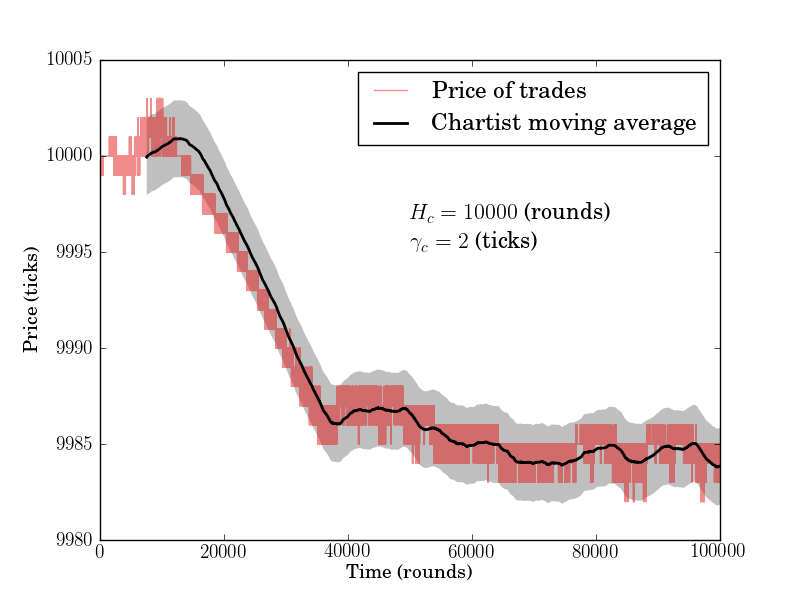
\includegraphics[width=0.5\textwidth]{agent_strategies/marketmaker/d.png}}
\subcaptionbox{}
[0.49\linewidth]{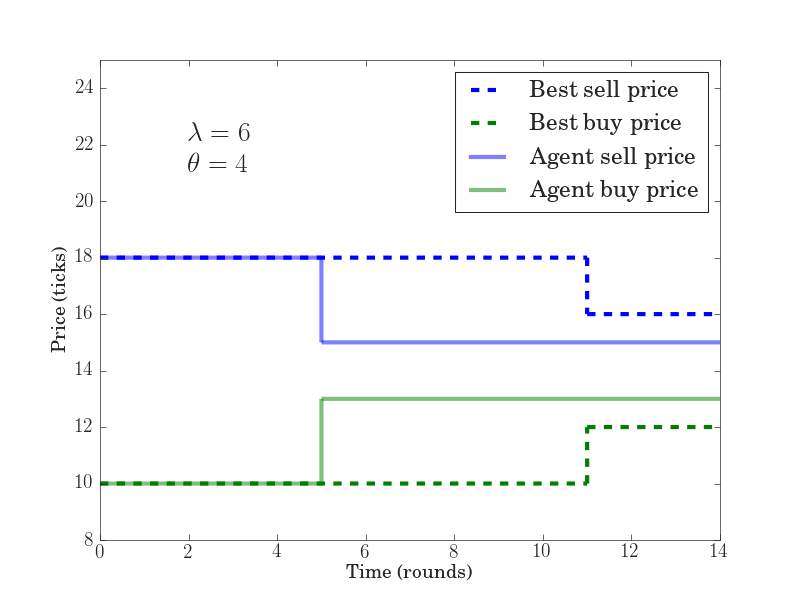
\includegraphics[width=0.5\textwidth]{agent_strategies/marketmaker/b.png}}
\subcaptionbox{}
[0.49\linewidth]{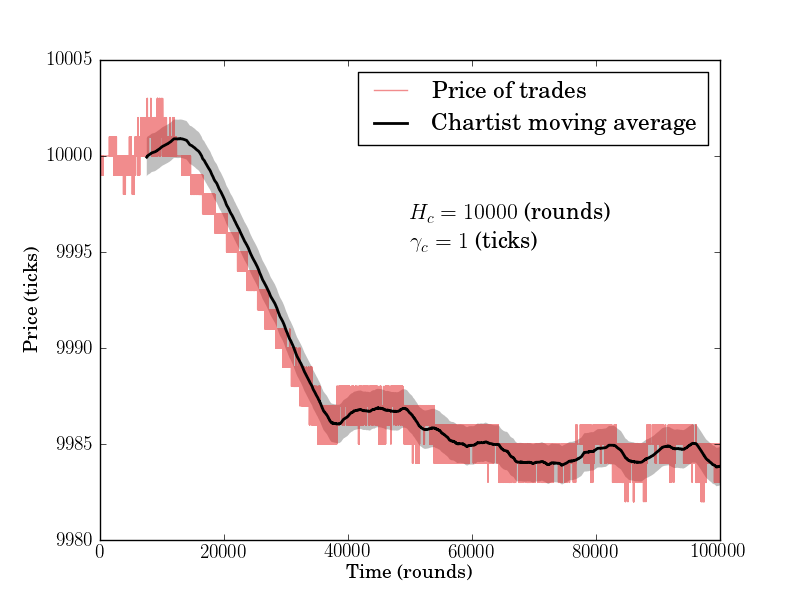
\includegraphics[width=0.5\textwidth]{agent_strategies/marketmaker/c.png}}
\caption{Examples illustrating the how the market maker updates its prices}
\label{figure:marketmaker_strategy}
\end{figure}


\subsubsection{Decision cycle}\label{section_tradeCycles}
Any market maker \marketmaker{i} be thought of as having a trading cycle, the length of which depends on the parameters \ssmmlatencyagent{i} and \ssmmthinkagent{i}. 
\begin{description}
\item[Acquire market information] The agent requests market information at round \round{T_0}. The request reaches the market at round $\round{T_0} + \ssmmlatencyagent{i}$, and the market instantly sends out a reply.
\item[Evaluate market information] The agent receives the market information at round $\round{T_0} +  2\ssmmlatencyagent{i}$, and evaluate its strategy. 
\item[Execute trade decision] The agent reaches a conclusion on how to trade at round $\round{T_0} + 2\ssmmlatencyagent{i} + \ssmmthinkagent{i}$, and sends off an order to the market. The order reaches the market at round $\round{T_0} + 3\ssmmlatencyagent{i} + \ssmmthinkagent{i}$.
\end{description}
As soon as \marketmaker{i} has submitted the new order, it also submits a new request for market information. The agent receives this second batch of market information at round $\round{T_0} + 3\ssmmlatencyagent{i} + \ssmmthinkagent{i}$, and the cycle restarts. The length of the cycle of \marketmaker{i} is therefore defined as
\begin{equation}
\marketmakercyclelength{i} = 3\ssmmlatencyagent{i} + \ssmmthinkagent{i}
\end{equation}
The length of the cycle is important for several reasons. First of all, since the market only requests new market information once during the cycle, the market maker observed the changes in the market with a frequency of $\frac{1}{\marketmakercyclelength{i}}$. Any market events that take place within a period smaller than \marketmakercyclelength{i} can be only partially observed by the market maker.

Secondly, since the market maker can only have a single order on each side of the order book, the latency to the market decides how much volume the market maker is able to buy and sell over a period of time. The market maker $i$ submits orders with a fixed volume \ssmmordervolumeagent{i} and the volume that the agent can supply the market with therefore depends on how much of the time the market maker manages to have standing orders at the market.

When an order submitted by the market maker is filled, the market sends out a transaction receipt which takes \ssmmlatencyagent{i} rounds to reach the market maker. When the market maker receives the receipt, the agent restarts the cycle by submitting a request for market information in order to submit a new order. This means that a total number of $4\ssmmlatencyagent{i} + \ssmmthinkagent{i}$ will elapse from time time that the order was filled to the time when the market maker can have another order placed in the order book. During this time, the market maker does not have an order in the market on the side of the book that the filled order was at. When the market maker does not have a standing order on either side of the book, it means that the agent does not contribute to increasing the liquidity of the asset. Hence, in this simple model, fast market maker should do a better job of supplying liquidity than slow market makers.




%Since it takes $\lambda_n$ rounds for the trade message to reach the market, the total time between the time of the agent requesting market information and the time at which the trade message arrives at the market, is $\round = 3\lambda_n + \lambda_d$. Hence shaving one round of speeds up the entire process of submitting a round by three rounds. 


\subsection{HFT Chartists}\label{section:hft_chartist}
The slow traders do not directly incorporate a chartist element into their strategy, as any changes in the traded price that occurs in the short time that the model simulates would be undetected by the slow traders. However, in order to incorporate chartist behavior in the model, a fast trader agent using a chartist strategy was implemented. These agents will from now on be referred to as HFT chartists, or simply as chartists. 
\subsubsection{Strategy outline}
The chartists use a simple strategy, in which they continually calculate the moving average of the traded prices over a time windows \cite{izumi2009evaluation}. If the current price drops below the moving average, the chartist believes that it has detected a downtrend. The chartists believes that the downtrend will continue for a while, and it will therefore try to get rid of any shares that it is currently holding. In order to accomplish this, the chartists starts to submit sell orders. The more urgently the agent is trying to sell its stocks, the lower it will set the price of the sell order, as a sell order at a lower price is more likely to be filled. On the other hand, if current price rises above the moving average, the agent believes that it has detected an up-trend, and that the stock will be worth more in the near future. The agents therefore starts to submit buy orders starts to submit buy orders at a higher price. The more strongly the agent believes in the stock price increasing, the higher it is willing to set the buy price. The agent only submit orders when it has detected a trend. As long as the chartist does not detect a trend, the agent is inactive and merely observes the market data.  After submitting an order, the agent waits for a while, as a precaution against submitting too many orders which would make the agent incur great losses the trend detected by the agent turns out to be wrong. This mechanism is also a limiting assumption of the model instated in order to protect the market from a few market makers flooding the market with a hige number of orders. As another step towards preventing the order books from filling up with chartist orders that might never be filled, and thus slow down the execution of the simulation is to make the chartists submit limit orders.

\subsubsection{Parameterization}
The agent strategy is parameterized as follows. HFT chartist agent \chartist{j} has the following parameters:
\begin{description}
\item[Time horizon] The parameter \sctimehorizonagent{j} determines determines the width of the window over which the agent calculates the moving average. Larger values of \sctimehorizonagent{j} makes the agent use trade price data from further in the past and makes the moving average less responsive to sudden change, while lower values makes the moving average react faster to sudden movements in the price. 
\item[Sensitivity] The sensitivity of \chartist{j} is given by the parameter \scticksbeforereactingagent{j} and refers to the number of ticks that the moving average of the traded price must differ from the currently traded price before the chartist recognizes that it has detected a trend. The higher the value of \scticksbeforereactingagent{j}, the less often the chartist will detect a trend. In the case of $\scticksbeforereactingagent{j} = 0$, the agent will detect a trend whenever $M \neq \currentprice$, which will be true in the majority of rounds.
\item[Aggressiveness] One the chartist decides to trade, it needs to decide upon a price. The aggressiveness parameter \scpriceticksizeagent{j} controls how far from \currentprice that the agent will set the price. This parameter reflects the agents confidence in its own belief about the trend, and the willingness of the agent to trade at sub-optimal prices in order to obtain or sell off shares.
\item[Trading frequency] Once the chartist has detected a trend, it will continue trading for as long as the trend persists. The parameter \scwaitTimeBetweenTradingagent{j} limits the frequency with which the chartist can submitting orders by specifying the number of round that the agent waits before submitting another order.
\end{description}

\subsubsection{Strategy evaluation}
In round \round{T}, the agent calculates the moving average of the buy and sell prices by subtracting the prices that are no longer inside the windows specified by \sctimehorizonagent{}, and adding the the most recent prices. The agent then calculates the average mid-price $\bar{M}_\text{tot}$which is used in the trend detection.
\begin{equation}
\bar{M}_\text{tot} = \frac{1}{2\sctimehorizonagent{}} \bigg[\sum\limits_{n=\round{p}}^{\round{T}} (\bestaskprice{n} + \bestbidprice{n}) - \sum\limits_{n=\round{p} - \sctimehorizonagent{}}^{\round{T} - \sctimehorizonagent{}} (\bestaskprice{n} + \bestbidprice{n})\bigg]
\end{equation}
where \round{p} is the latest round in which the agent was previously active. The agent calculates the current mid-price $m$:
\begin{equation}
m = \frac{\bestaskprice{T} + \bestbidprice{T}}{2}
\end{equation}
The agent then uses a simple rule to decide whether to sell or buy, and at what price:
\begin{flalign}
&\text{Place a buy order if} & & m > \bar{M}_\text{tot} + \scticksbeforereactingagent{} && \text{at buy price} & & p = m + \scpriceticksizeagent{}\\
&\text{Place a sell order if}  & & m < \bar{M}_\text{tot} - \scticksbeforereactingagent{} && \text{at sell price} & & p = m - \scpriceticksizeagent{}
\end{flalign}


Figure \ref{figure:chartist_strategy} provides two examples of how the sensitivity parameter \scticksbeforereactingagent{} and the parameter for the time horizon of the chartist strategy \scticksbeforereactingagent{} influences when the agent will trade or not. In the left figure, the agent has a low sensitivity to price changes, as indicated by the narrow area shaded gray around the black line indicating the moving average calculated by the agent. Since $\scticksbeforereactingagent{} = 1$, the traded price only has to deviate by a single tick from the moving average before the agent will submit orders to trade. In this case, the agent uses a moving average calculated over a relatively short span of $\scticksbeforereactingagent{} = 5000$ rounds, which makes the moving average reflect short-lived price trends. As the figure shows, these parameters prompt the agent to detect trends more or less constantly, and the agent even detects a short up-trend in the beginning of the simulation, as is shown where the traded price (red) does not stay within the gray shaded area . In the right figure, the agent has a sensitivity of $\scticksbeforereactingagent{} = 2$ and a longer time horizon of $\scticksbeforereactingagent{} = 15000$ rounds. Consequently, the agent detects a downtrend in round 12000 or so, where the traded prices, and begins to submit sell orders. However, just before round 40000, the agent decides that the downtrend has ended and the agent becomes inactive until the next time a trend is detected. 
\begin{figure}
%issue 11
\subcaptionbox{\label{subfig:}}
[0.49\linewidth]{\includegraphics[width=0.5\textwidth]{agent_strategies/chartist/a.png}}
\subcaptionbox{\label{subfig:}}
[0.49\linewidth]{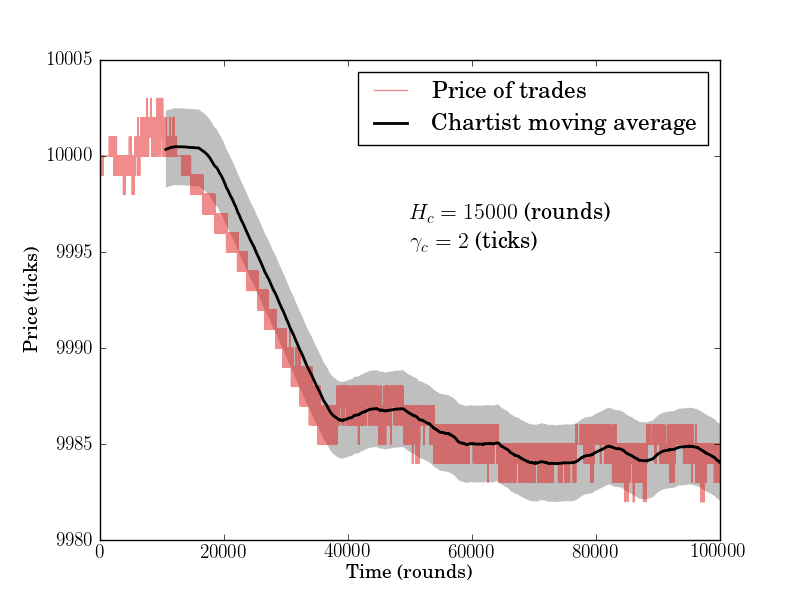
\includegraphics[width=0.5\textwidth]{agent_strategies/chartist/h.png}}
\caption{Examples illustrating the chartist decision strategy}
\label{figure:chartist_strategy}
\end{figure}





\begin{comment}
\subsubsection{Fundamental price}\label{section:fundamental_price}
A common way to model the development of the fundamental price is to use a stochastic random walk process. The idea is that, assuming that markets are efficient, any available information about the stock is already reflected in the fundamental price. When some news arrive, this will quickly cause the price to change according to the nature of the news, as rational traders act to adapt to the new situation. The justification for modeling this with a random walk is that, since the fundamental price already reflect whatever news is available, it will only change as new information is released. In other words, the fundamental price is independent of past information. Since new information is fundamentally unpredictable, a random walk model seems suitable. 


\begin{figure}
%issue 11
\subcaptionbox{\label{subfig:}}
[0.49\linewidth]{
\includegraphics[width=0.5\textwidth]{Electron.pdf}}
\subcaptionbox{\label{subfig:}}
[0.49\linewidth]{
\includegraphics[width=0.5\textwidth]{Electron.pdf}}
\caption{\textbf{:}}\label{fig:}
\end{figure}
content...
\end{comment}

%\section{Implementation}


%\section{Overview of model parameters}\label{section:overview_of_model_parameters}



